
	\begin{figure}	
		\begin{subfigure}{3.5cm}
			\begin{align*}
			F   = & \{a, b, c \}           \\
			N_p = & \{A, B, C\}      \\
			N_c = & \{AC, T_I\}            \\ 
			M   = & \{  (T_I, \{AC, B\}), \\
			&    (AC, \{A, C\})  \} \\
			S_I = & \{ a \} 	             \\ 
			\end{align*} 
		\end{subfigure}		
		\scalebox{0.6}{
			\begin{subfigure}{7cm}
				\begin{tikzpicture}[auto,node distance=1.5cm,
				thick,main node/.style={circle,draw,font=\sffamily\Large\bfseries},
				square node/.style={rectangle,draw,font=\sffamily\Large\bfseries}]
				\node[] (InitState) {}; %{ $\mathbf{S_I = \{a\}}$ };
				
				\node[main node] (Init) [right=3cm of InitState] {$T_I$};
				\node[main node] (AC) [right=2cm of Init, below of=Init] {$AC$}; 
				
				\node[main node] (A) [below left = 2em and 2em of AC] {$A$};
				\node[main node] (B) [below left = 2em and 2em of Init] {$B$}; 
				\node[main node] (C) [below right = 2em and 2em of AC] {$C$}; 
			
				\path[every node/.style={font=\sffamily\small}]
				(Init) edge [->] node [left] {} (B)
				(Init) edge [->] node [left] {} (AC)
				(AC) edge [->] node [left] {} (A)
				(AC) edge [->] node [left] {} (C);
				\end{tikzpicture}
			\end{subfigure}	
		}	
		\caption{Diagram showing an example problem and its decomposition.}	
	\end{figure}
	
	\begin{figure}
		\scalebox{0.8}{
			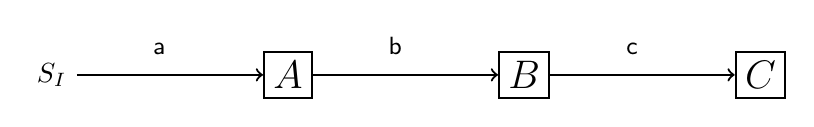
\begin{tikzpicture}[auto,node distance=3cm,
			thick,main node/.style={circle,draw,font=\sffamily\Large\bfseries},
			square node/.style={rectangle,draw,font=\sffamily\Large\bfseries}]
			
			\node[] (Invis) [] {$S_I$};
			\node[square node] (A) [right of=Invis] {$A$};
			\node[square node] (B) [right of=A] {$B$};
			\node[square node] (C) [right of=B] {$C$};
			
			
			\path[every node/.style={font=\sffamily\small}]
			(Invis) edge [->] node [left, label=a] {} (A)
			(A) edge [->] node [left, label=b] {} (B)
			(B) edge [->] node [left, label=c] {} (C);
			\end{tikzpicture}		
		}
			\caption{The only possible solution $A, B, C$ for E.g.\ 1, requires the children of $AC$ and $B$ to be interleaved, meaning we cannot impose an order between them}
	\end{figure}
	
	


\section{Related Work}
% FROM (https://ojs.aaai.org/index.php/ICAPS/article/view/15944/15755) A Closer Look at Causal Links: Complexity Resultsfor Delete-Relaxation in Partial Order Causal Link (POCL) Planning
Our linearization procedure is a pre-processing technique for the search space, is a compilation of an HTN planning problem class to a different class of problems, and can exploit specialised TO planners.

The panda$_\pi$ grounder by \cite{Behnke2020Grounding} also prunes unreachable tasks, methods, etc.\.  Because the panda$_{\pi}$ planner is a grounded planner, we can ground then linearize, or vice-versa to \enquote{stack} the reduction in search space. 

The main optimization of HyperTensioN by \cite{hypertension} is via the Pullup extension - which determines additional preconditions of methods and compound tasks by analysing the preconditions of possible child actions. Unlike ours, no approximation of effects are considered.  


The HTN2STRIPS planner by \cite{HTN2STRIPS} and HTN2SAS planner by \cite{HTN2SAS} compiles HTN problems, both totally and partially ordered, to classical problems. The TOAD planner by \cite{HollerTOAD} compiles TOHTN problems into classical planning problems in order to allow the use of classical planning systems. The panda$_\pi$ engine progression search configuration, also uses a compilation to classical problems.
% TOAD over-approximates the set of solutions to the HTN problem. In the empirical evaluation the paper performed, TOAD achieved higher coverage than the base version of HTN2STRIPS, and all systems submitted to the totally ordered track of the 2020 IPC.  

There exists totSAT planner by \cite{TOtoSAT} that compiles a totally ordered problem to SAT problem. There also exists 2 planners by \cite{POtoSAT, OptimalPOtoSAT} that compiles a partially ordered problem to a SAT problem. One searches for optimal plans, the other focuses on finding any solution as quickly as possible. Lilotane by \cite{Lilotane} directly encodes a lifted problem representation into a SAT problem.

Another planner by \cite{Behnke_Speck_2021} converts TOHTN into Binary Decision Diagrams (BDDs), then use symbolic search on it.

The BDD planner by \cite{Behnke_Speck_2021}, totSAT planner by \cite{TOtoSAT}, TOAD by \cite{HollerTOAD}, HyperTensioN by \cite{hypertension}, and Lilotane by \cite{Lilotane}, as discussed before, are all specialised TO planners. So are the TFD (Totally Ordered Fast Downward) and PFD (Partially Ordered Fast Downward) hierarchical planners by \cite{PDDL4J}.  Note however that HTN2SAS achieved similar coverage than greedy search with panda$_\pi$, a partial-order planner.
